% fig_mho_rxplane.tex
% R-X impedance plane showing three Mho zones and key operating points
% Z_line = j0.05 pu, MTA=80°
% Zone 1: 80% = j0.040; Zone 2: 120% = j0.060; Zone 3: 180% = j0.090
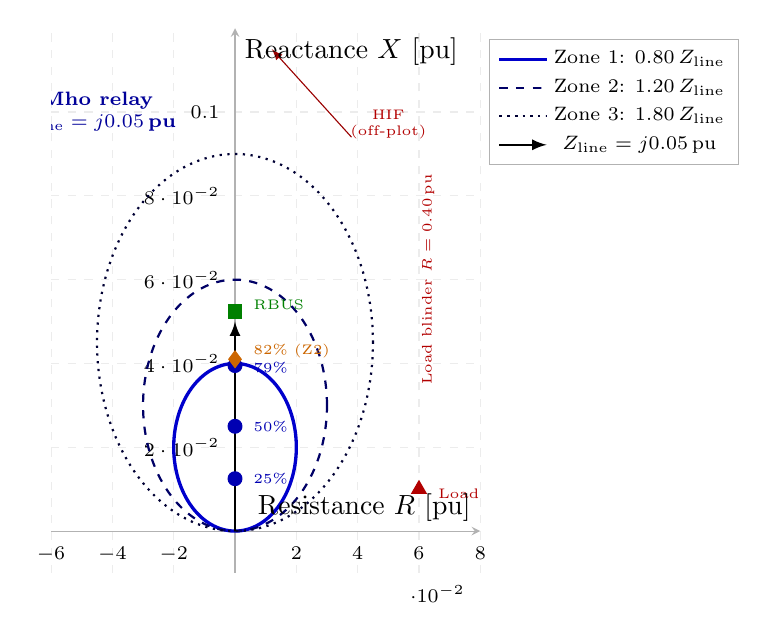
\begin{tikzpicture}
\begin{axis}[
  name        = rxax,
  width       = 0.58\textwidth,
  height      = 8.5cm,
  xlabel      = {Resistance $R$ [pu]},
  ylabel      = {Reactance $X$ [pu]},
  xlabel style= {font=\small},
  ylabel style= {font=\small},
  xmin=-0.06, xmax=0.08,
  ymin=-0.01, ymax=0.12,
  xtick       = {-0.06,-0.04,-0.02,0,0.02,0.04,0.06,0.08},
  ytick       = {0,0.02,0.04,0.06,0.08,0.10},
  xticklabel style={font=\scriptsize},
  yticklabel style={font=\scriptsize},
  axis lines  = center,
  axis line style={gray!60},
  tick style  = {draw=none},
  grid        = major,
  grid style  = {gray!15, dashed},
  legend style={at={(1.02,0.98)}, anchor=north west,
                font=\scriptsize, draw=gray!60, fill=white},
]

% ---- Mho circles (self-polarised, MTA=90° simplification for reactive line)
% Zone 1: centre=(0, 0.020), radius=0.020
% Zone 2: centre=(0, 0.030), radius=0.030
% Zone 3: centre=(0, 0.045), radius=0.045
\addplot[blue!80!black, very thick, smooth, domain=0:360, samples=200]
  ({0.020*cos(x)}, {0.020 + 0.020*sin(x)});
\addlegendentry{Zone 1: $0.80\,Z_{\rm line}$}

\addplot[blue!40!black, thick, dashed, smooth, domain=0:360, samples=200]
  ({0.030*cos(x)}, {0.030 + 0.030*sin(x)});
\addlegendentry{Zone 2: $1.20\,Z_{\rm line}$}

\addplot[blue!20!black, thick, dotted, smooth, domain=0:360, samples=200]
  ({0.045*cos(x)}, {0.045 + 0.045*sin(x)});
\addlegendentry{Zone 3: $1.80\,Z_{\rm line}$}

% ---- Z_line (positive-sequence line impedance locus) -----------------------
\addplot[black, thick, -latex, samples=2, domain=0:0.05]
  ({0}, {x});
\addlegendentry{$Z_{\rm line}=j0.05$\,pu}

% ---- Key operating points --------------------------------------------------
% INT_25: d=0.25 → Z_m=j0.0125
\addplot[mark=*, mark size=2.5pt, blue!70!black, only marks]
  coordinates {(0, 0.0125)};
\node[font=\tiny, blue!70!black, right=1pt] at (axis cs:0.002, 0.0125) {25\%};

% INT_50: d=0.50 → Z_m=j0.025
\addplot[mark=*, mark size=2.5pt, blue!70!black, only marks]
  coordinates {(0, 0.025)};
\node[font=\tiny, blue!70!black, right=1pt] at (axis cs:0.002, 0.025) {50\%};

% INT_79: d=0.79 → Z_m=j0.0395 (just inside Zone 1)
\addplot[mark=*, mark size=2.5pt, blue!70!black, only marks]
  coordinates {(0, 0.0395)};
\node[font=\tiny, blue!70!black, right=1pt] at (axis cs:0.002, 0.039) {79\%};

% INT_82: d=0.82 → Z_m=j0.041 (Zone 2 only)
\addplot[mark=diamond*, mark size=3pt, orange!80!black, only marks]
  coordinates {(0, 0.041)};
\node[font=\tiny, orange!80!black, right=1pt] at (axis cs:0.002, 0.043) {82\% (Z2)};

% Remote bus: d=1.05 → Z_m=j0.0525
\addplot[mark=square*, mark size=2.5pt, green!50!black, only marks]
  coordinates {(0, 0.0525)};
\node[font=\tiny, green!50!black, right=1pt] at (axis cs:0.002, 0.054) {RBUS};

% HIF: ag with Z_arc=j1.5 → Z_m=j2.275 (outside all zones, off-plot)
% Show as an arrow indicating out-of-zone
\node[font=\tiny, red!70!black, align=center]
  at (axis cs:0.05, 0.097) {HIF\\(off-plot)};
\draw[-latex, red!60!black]
  (axis cs:0.038, 0.094) -- (axis cs:0.012, 0.115);

% ---- Load blinder boundary -------------------------------------------------
\addplot[red!60!black, thick, dashed, samples=2, domain=-0.01:0.12]
  ({0.40}, {x});   % x=0.40 off the plot → just show label
\node[font=\tiny, red!70!black, rotate=90]
  at (axis cs:0.063, 0.06) {Load blinder $R=0.40$\,pu};

% Load point: (0.5, 0.1) — outside blinder line (off to right)
\addplot[mark=triangle*, mark size=3pt, red!70!black, only marks]
  coordinates {(0.06, 0.010)};
\node[font=\tiny, red!70!black] at (axis cs:0.073, 0.009) {Load};

% ---- Labels ----------------------------------------------------------------
\node[font=\scriptsize\bfseries, blue!60!black, align=center]
  at (axis cs:-0.045, 0.100) {Mho relay\\$Z_{\rm line}=j0.05$\,pu};

\end{axis}
\end{tikzpicture}
